
\chapter{Related Work}

In this chapter we will give a brief overview over different services offered in the Web, to point out what services in the Web all can be.
We then introduce the Event-Condition-Action (\textrm{ECA}) paradigm, an event-driven approach to impose reactivity.
And finally we point out existing rule languages and engines that exploit the \textrm{ECA} paradigm.



\section{Services in the Web}
\index{Web Service}
\index{Services}
\index{World Wide Web}

The term service in the context of the Web is ambiguous and there have been a lot of different approaches to offer services within the Web.
For example the term \textrm{Web Services} often refers to interfaces that are used in the \textrm{World Wide Web} for communication between applications.
We will point out some main research areas on service-orientation within the Web.

Remote execution of programs on other computers has always been a strong research area. And with the coinage of the term \textrm{World Wide Web}~\cite{DBLP:journals/en/Berners-LeeCGP92}, there were also trends towards services offered through the Web; computers waiting in the Web for a request in order to execute some application logic and return an answer.
\index{SOA}
The encapsulation of functionality into services~\cite{peltz2003web} in order to offer them to other applications is called service-oriented architecture (\textrm{SOA})~\cite{perrey2003service}.
Adopting \textrm{SOA} internally to an application means splitting the application into smaller pieces, which then communiacte via these services among each other.
This does not only provide robustness, it also allows the reuse of functionality through services.
Moreover these services can be offered to other applications and also to the Web, thus allowing others to access certain functionalty or even the whole application.
All nodes in the Web are stand-alone entities, which offer services of some sort, be it a webpage, data, instant measurements or functionality.
This makes the Web itself a service-oriented architecture and all these services are naturally services in the Web.
It is for its advantages that \textrm{SOA} has received a great deal of attention and has been widely adopted, mostly throughout the Web.
This lead to an increasing number of Web accessible services and their compositions, the so called \textrm{Mashups}.
An empirical study~\cite{conf/icws/HuangFT12} on a directory, which they call the \textit{"[...] most active Web APIs and mashups collection"}, and data taken from this resource (depicted in Figure \ref{fig:NumOfAPIs}) seem to underline a growing popularity, at least in terms of publishing services through this directory.

\begin{figure}[!ht]
  \centering
  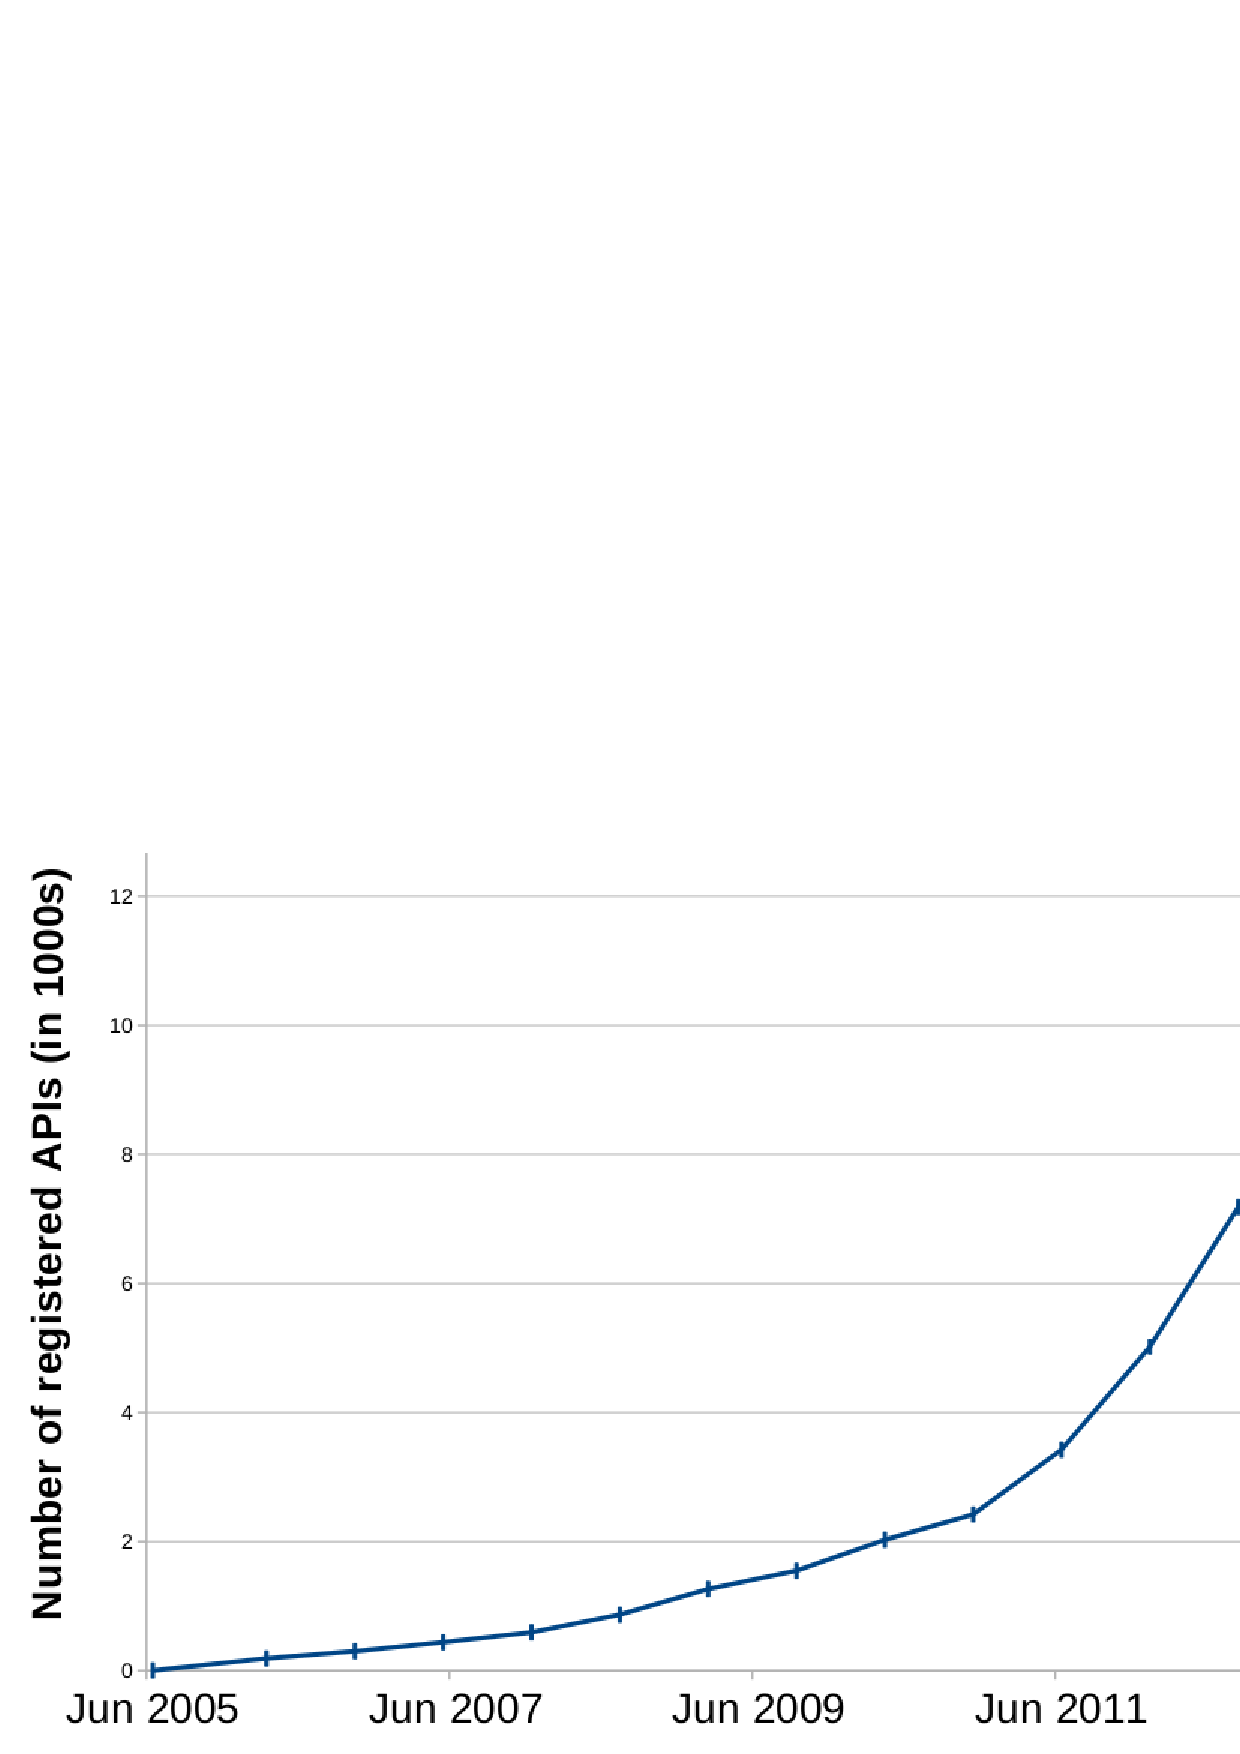
\includegraphics[width=0.55\textwidth]{figures/NumOfAPIs}
  \caption{Number of registered APIs in the ProgrammableWeb directory by date}
  \label{fig:NumOfAPIs}
\end{figure}


\subsection{Requesting Services in the Web}
\index{RPC}
An early adoption of the service concept to computers were the Remote Procedure Calls (\textrm{RPC})~\cite{Birrell:1984:IRP:2080.357392}.
Through \textrm{RPC} a piece of code can be executed on a different machine, than the one which is calling the procedure.
It is basically achieved via inter-process communication and doesn't necessarily require the Web.
Even more since when \textrm{RPC} was invented, the \textrm{World Wide Web} wasn't even postulated by Tim Berners-Lee. 
\textrm{RPC} also found its use in grid computing~\cite{seymour2002overview} and through this, opened doors into the field of distributed computation.
The \textrm{RPC} paradigm isn't bound to certain technologies and thus, has been implemented in a lot of differrent programming languages.
These implementations were tightly bound to the respective language that was used, which resulted largely in incomptaiblity among them.
\index{XML}
\index{XML-RPC}
It became necessary to enhance \textrm{RPC}'s in order to get cross platform compatibility.
By abstracting \textrm{RPC} functionality with the Extensible Markup Language (\textrm{XML})~\cite{bray1998extensible}, compatibility between services that used different technologies was easier to achieve.

\index{SOAP}
\index{WSDL}
Since \textrm{XML-RPC} was held relatively simple but received a lot of attention, it was further enhanced.
Together with additional proposedy functionality, XML-RPC heavily influenced Simple Object Access Protocol (\textrm{SOAP})~\cite{box2000simple}.
\textrm{SOAP} is accompanied by the Web Service Description Language (\textrm{WSDL})~\cite{christensen2001web} which is used to describe the interfaces to SOAP services.
Through \textrm{SOAP} and \textrm{WSDL} a client for the service can issue a request for the \textrm{WSDL} information of the service and retrieves all interface specifications he requires in order to issue a call to the actual service.
The service specifications are then incorporated into the existing application as if it is a local function call.
\textrm{SOAP} has found its applicability in business applications~\cite{journals/itpro/BarrosD06} and was enhanced with a lot of industrial standards, also called the "WS-*" specifications, e.g. WS-Addressing, WS-Policy or WS-Security.

\index{CORBA}
Another initiative that aimed for eased communication between different platform is the Common Object Request Broker Architecture (\textrm{CORBA})~\cite{dec1991common}.
As the name already suggest it is an object-oriented approach and it allows the exchange of whole objects.
\index{ORB}
\textrm{CORBA} relies on its communication layer, the Object Request Broker (\textrm{ORB}), which forms the basis of its architecture.
The platform-specific \textrm{ORB}'s provide the communication abstraction, which free the application from platform dependencies.
\index{IDL}
Similar to \textrm{SOAP}'s \textrm{WSDL}, \textrm{CORBA} has its Interface Definition Languange (\textrm{IDL}) to provide information about the objects to be offered and accessed.
An object is instantiated by an application and the interface to this instance is offered through the \textrm{ORB}.
Another application attached to the \textrm{ORB} can then access all public variables, data structures and functions of this object.
This means not only remote access to variables and data structures, but also remote function invocation.
\textrm{CORBA} requires the implementation of object-oriented mechanisms in programming languages which aren't object-oriented.
This can be technically difficult and become an eventually tedious task.
\textrm{CORBA} allows communication between applications written in different programming languages and which are running on the same physical computer, as well as the communication between different computers in the same network.
With the Internet Inter-\textrm{ORB} Protocol (\textrm{IIOP}) it is also possible to connect \textrm{ORB}'s over the Web.
Through this, the offered objects can become services in the Web, but they are shielded by the \textrm{ORB}.

\index{REST}
All the afore mentioned approaches require a specific protocol and are therefore incompatible with each other.
For this reason and its simplicity, an architectural style has gained popularity which frees application from this constraint: Representational State Transfer (\textrm{REST})~\cite{fielding2000architectural}.
\textrm{REST} concentrates on the roles of components and on constraints upon interactions between them.
An important architectural constraint is that all communication is stateless, which means for a client-server communication, no state is stored on the server.
Therefore all informations required for a single interaction need to be provided within one request.
This allows for the definition of simple and well-defined interfaces, since responses are not bound to a certain session state. 
\index{REST}
Services within the Web that adhere to the \textrm{REST} architecture are called \textrm{RESTful} Web services.
Simple access to services without communication overhead and required negotiation before using it, increased \textrm{REST}'s popularity and spread it into more application fields.
There is for example the upcoming concept of the \textrm{Web of Things}~\cite{Guinard2011WoT}, which aims to incorporate smart things (e.g. tagged things, sensor measurements, device controllers, etc.) into the Web through \textrm{REST} interfaces.
\textrm{REST} brings advantages into the context of smart things connected to the Web, because incompatible standards and protocols were used by different manufacturers of such things.


\subsection{Composing Services in the Web}
% \section{Weakening the Relevance of the Client-Server Model}
% \textit{Dropping the Client-Server Model}\\
% \textit{The Interweavement of Client and Server}\\
Webpages emerged into dynamic sites on the web through the upcoming of scripting languages to control the browser and the webpage itself.
With all their infrastructure in the background on the server they became literally applications.
\index{Web Application}
These Web applications (\textrm{Web Apps}) went even more responsive with the advent of asynchronous calls from the browser to the server, which allows to load data into the current webpage while the user is interacting with it.
\index{API}
\index{Web API}
Those asynchronous calls are requests to services, which act as the application programming interface \textrm{API} to the \textrm{Web App} (\textrm{Web APIs}) which sits on the server.
As a side-note, the term \textrm{Web API} not only comprises server-side interfaces but also client-sided ones (e.g. the browser), after all they are also interfaces to the Web.
For server-side \textrm{Web APIs} this means that these services can be accessed from other entities in the Web than just browsers, which eases application to application communication.
Basically a \textrm{Web App} can be controlled without the user interface, which is often delivered by the provider of the application.
Imagine not going to the Google webpage anymore to make a search and crawling through the results, but you have your own application doing it for you and processing the results instantly.
There is a trend of \textrm{Web App} providers to publish their \textrm{Web API} in order to grant easy access to it.
This lead to an increase of the number of \textrm{Web App Mashups} in the past few years.

\index{Mashup}
\textrm{Mashups} combine data and functionality of more than one service in the Web in a new site.
Simple services from different sources can be combined into more powerful ones, which can in turn again be composed and so on.
These service compositions assemble data and services in a novel way which provides a new perspective.
Ever since services were accessible in a more or less convenient way, \textrm{Mashups} have been developped as well.
On of the first Web service \textrm{Mashups}~\cite{wwwHosuingMaps}, was invented in the same year after Google Maps came up in 2005.
It was a webpage that displayed CraigsList's rental houses on a Google Map.
At that time no \textrm{Web API} was available that provided easy access to these two services, but there was an advantage to be seen from everybody being able to create a \textrm{Mashup} through publicly available services.
Such \textrm{Mashups} are often a read-only fixed wiring of different services that provide a new view on specific data.
Some recent \textrm{Mashup} examples, taken from the \textrm{ProgrammableWeb}~\cite{wwwProgrammableWeb} collection, are:

\begin{itemize}
  \item \textrm{Wifi and Plugs}: MapBox, Google Docs and Import.io API's used to display where Wi-Fi and plugs are available in London.
  \item \textrm{MapLight}: GovTrack.us and OpenSecrets API's used to combine political results with financial contributions to show how capital contributions to influence politics affect voting.
  \item \textrm{Shared Count}: Facebook, LinkedIn, Pinterest and Twitter API's used to display informations about how well spread a URL is on social media sites.
\end{itemize}

But there are also efforts in research~\cite{10.1007/978-3-642-22233-7_11}\cite{4278815}\cite{Rizzotti:2010:UST:1772690.1772861}\cite{Stolee20131289} for flexible \textrm{Mashups}, where users are capable of choosing what and how to link in order to enhance Web resources according to their needs.
These flexible \textrm{Mashup} applications often provide methods to access user-specific functionality within \textrm{Web Apps}, which makes them even more user-centered and customizable.


\subsection{Subscribing to Services in the Web}
There is another type of service in the Web which is quite the opposite to the afore mentioned approches in terms of the data flow.
\index{Webhooks}
\textrm{Webhooks} are a method that enables the asynchronous delivery of data whenever it gets available, compared to the need of actively requesting a service to deliver it.
They are unifrom resource identifiers (\textrm{URI}), which point to a service in the Web, which accepts the data delivered to it.
% ~\cite{Eugster:2003:MFP:857076.857078}
Within the publish/subscribe pardigm, such asynchronous delivery of data is referred to as events, since that's what the appearance of new data is.
\textrm{Webhooks} are callbacks that can be placed by a \textrm{Web App} provider or a user at a remote location, informing the data prolifering site about their interest in the data.
Both parties are services in the Web, since the \textrm{Webhook} providers accept the data delivered to their \textrm{URI} and the \textrm{Webhook} receipients offer to send the data.


\subsection{Towards Simple Access and Communication}
\index{JSON}
With JavaScript's success as browser scripting language and recently also as server-side programming language, JavaScript Object Notification (\textrm{JSON}) as an alternative to \textrm{XML} has become popular for data representation throughout the Web.
It is also because of its human-readable format and often simple parsing into data structures of existing programming languages.
There is a notable trend towards \textrm{RESTful} services in the Web that offer \textrm{JSON} communication.
\index{Web Programmability}
They benefit from simple but powerful interfaces and easy to debug human-readable communication, which eases integration into other applications, along with the reduced communication volume.
Together with client- and server-side \textrm{Web APIs} the Web becomes ever more programmable.
% Figure \ref{fig:slide-11-1024} shows how the previously mentioned \textrm{ProgrammableWeb} directory experiences this trend as there were almost five times more \textrm{RESTful} services registered compared to \textrm{SOAP} services.
% An interesting point in this figure is that they label it \textrm{REST}, but this wouldn't exclude any of the other protocols, because the architecture behind them could also adhere to \textrm{REST}.
% We assume
% \begin{figure}[!ht]
%   \centering
%   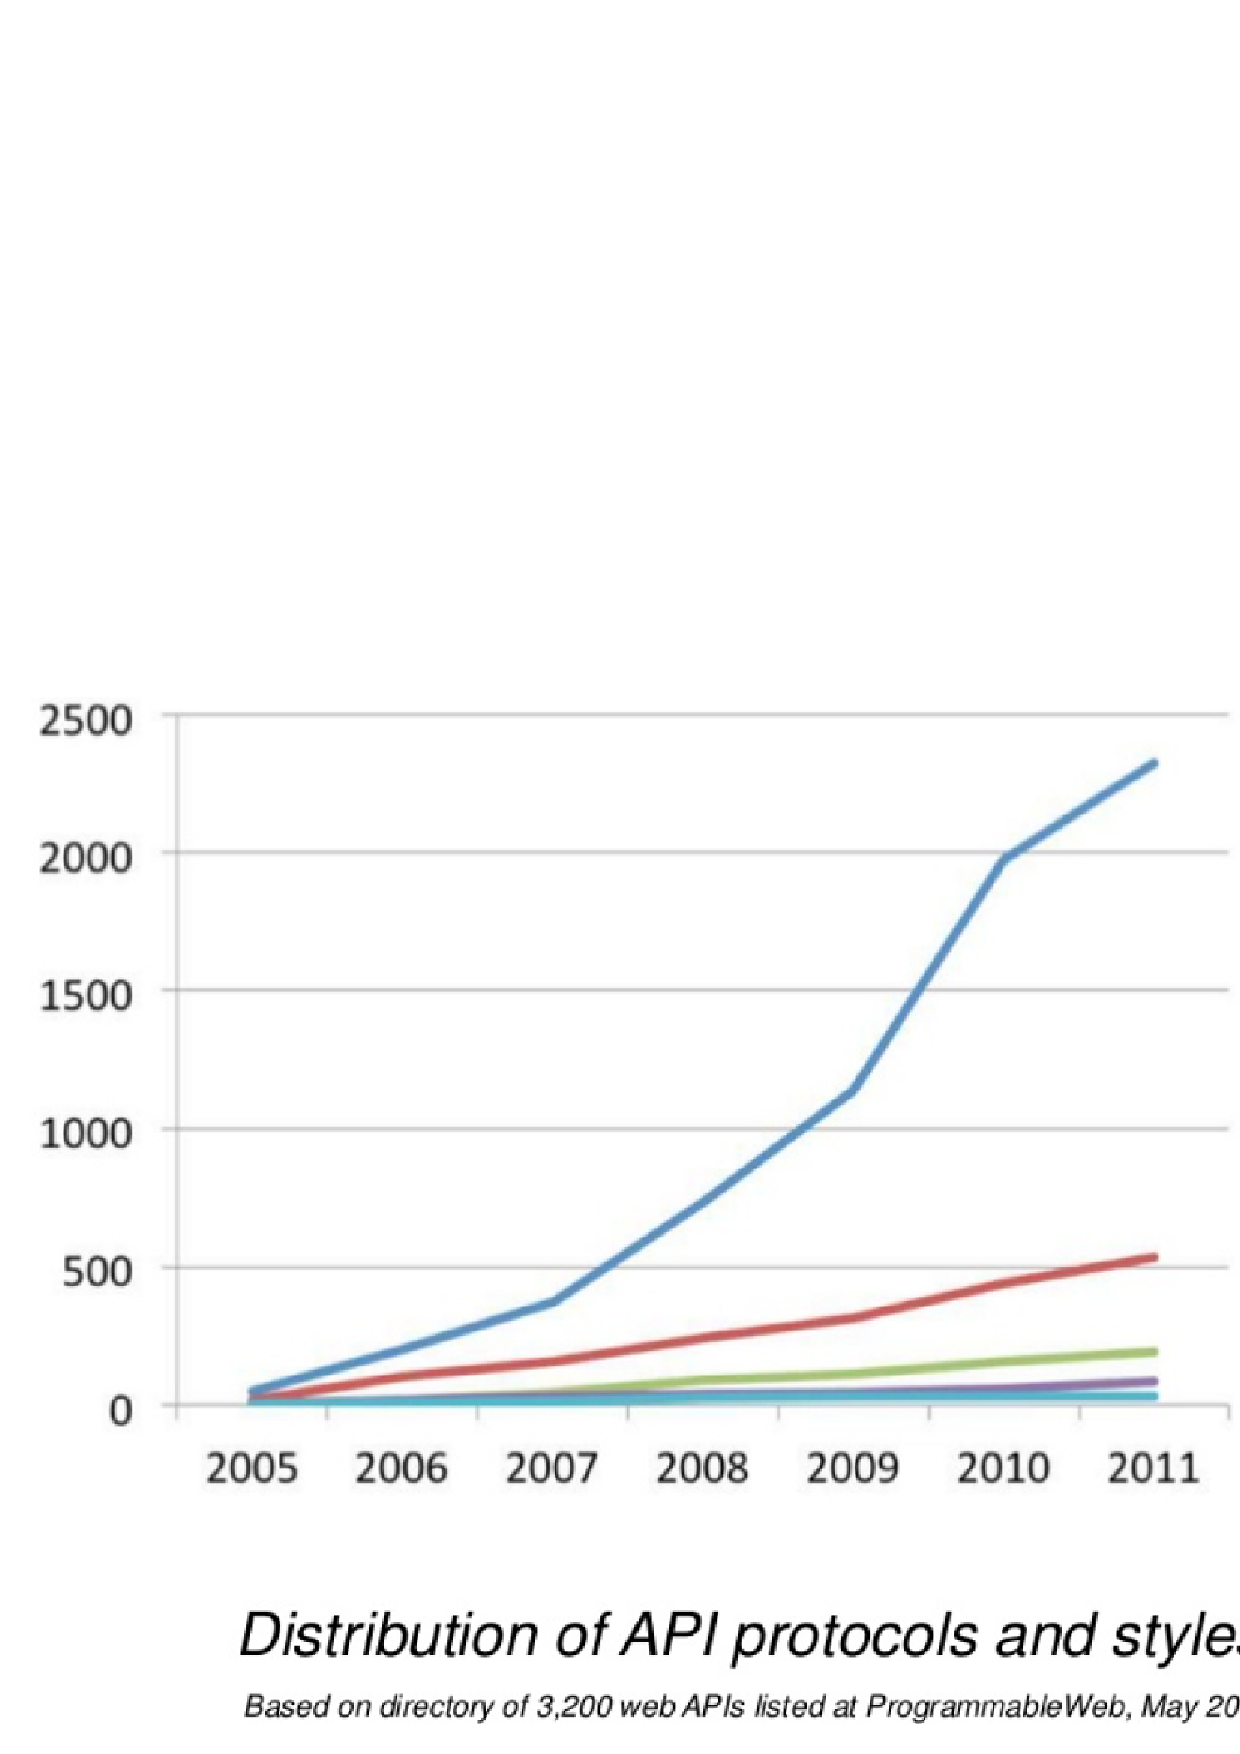
\includegraphics[width=0.6\textwidth]{figures/slide-11-1024}
%   \caption{REST vs. SOAP: Simplicity wins again\\(John Musser, ProgrammableWeb, 2011)}
%   \label{fig:slide-11-1024}
% \end{figure}


\section{Reactivity through Event-Condition-Action Rules}
\index{ECA}
We have shown research in different areas that lead towards a programmable Web.
As a result of this research, it is getting easier to compose and orchestrate services in the Web, but it still requires a lot of expertise or the suffering of limitations.
A considerable amount of literature~\cite{2007_AlferesR3}(!IMPORTANT!)\cite{2005-Bry_etal-XChange.pdf}\cite{10.1007-11896548_63}\cite{2012-Paschke_etal-ReactionRuleML.pdf} has been published on reactivity.
These studies underline that Event-Conditon-Action (\textrm{ECA}) rules are a powerful way to impose reactivity.
the concepts f an eca rule lnguage have been well studied. 
Such rules consist of three parts:
\begin{itemize}
  \item Event:
  \item Condition:
  \item Action:
\end{itemize}
 [2][3][11][12][23]
All research funneled into RuleML


\section{Rule Engines \& Rule Languages}
\index{Rule Engine}
\index{Rule Language}

It turns out that Web App mashing up is not able to bring reactivity to the Web.
They are merely aggregations of services, which only provide data or functions but no write possibilities such as Web applications provide.
% only subset of accesible functionalty/parametrization is provided


%TODO Table with categorization of Rule languages
% show rule engines, alsoo CEP, describe event composition through templates and why we don't do it

Several different rule languages have been developped for different purposes over the last years and they vary grately in their purpose.
% terms of usability for ECA Rules together with Web API mashups.
We examined different existing rule languages with respect to a certain use case to identify its applicability for reactivity in the Web. % TODO find other word as applicability
The use case is defined such that the rule needs to suffice the ECA paradigm:
In Appendix \ref{lst:JSONEvent}
In Appendix \ref{lst:myrdf}
\begin{itemize}
  \item Event: Receipt of an Email
  \item Condition: Check for a certain sender
  \item Action: Store it remotely via a Web API
\end{itemize}
Definition of events\cite{Adaikkalavan2007}




We defined an email event which the rule languages need to be able to process.
The JSON representation of the given email event as depicted in the appendix. %is shown in Listing~\ref{lstemail}.

% FIXME Leave out what was not inspiring!

\index{RDF}
\index{XML}
An early ECA Rule Language for XML repositories~\cite{Papamarkos03event-condition-actionrule} was postulated in 2003 and was picked up by many researches afterwards. It was designed to react on insert and delete events within XML repositories and as an action change XML documents.


Now apart from implementing a rules engine, we would also need to add an XML document event manager which interpretes and pushes events into the XML file \emph{inbound\_queue.xml}. Then again this instance would interprete the ouptuts of the ECA engine, which would theoretically manifest in other XML documents, and produce meaningful actions on remote hosts. This wouldn't be an architecture which has its focus on the solution of our use case and, as a result, add complexity and create an unnecessary overhead.

\index{Notation3}
To make the lengthy RDF definitions smaller and more readable, Notation 3~\cite{berners2006notation} was designed and announced in 2005. Through the implies operator(=\textgreater) an "event" can be connected to an "action", both expressed in RDF's subject, predicate, object notation, which makes the expression of ECA rules a complicated and not very intuitive task. A solution to our use case would look as follows:

This language is used to express relations between entities and thus not really suitable for our use case, since we would require another interpreter to infer the actions. But concepts and ideas of the work that was done in these consortias could eventually still find influence into our solution.

\index{XChange}\index{Xcerpt}
The rule language XChange~\cite{2005-Patranjan-TLE.pdf} was the outcome of the REWERSE (~\cite{wwwRewerse}, Reasoning on the Web with Rules and Semantics) project, which was funded by the EU and Switzerland. Their work influenced a number of future research. The language was designed to add reactive behaviour to a "static" Web which is represented through XML resources. Thus we have action logics to alter such resources through insertions and deletions. Since we aim to utilize Web API's for our rule language we need a more generic approach which adds flexibility in term of the API provided. But the thorough research done with the language XChange holds valuable concepts, especially in terms of temporal evet composition. This could be a rule according to our use case:


But XChange is designed to access other resources in an action and thus provides powerful tools:

\index{JSON Rules}
In 2008 \emph{JSON Rules}~\cite{2008-Giurca_Pascalau-JSON_Rules.pdf} was introduced as a language to easily react on specific DOM tree compositions.
The usage of JavaScript allowed them to provide simple functions which could be called directly by the actions, thus abstracting functionality from the language.
This key concept found influence into our language as it allows different layers of abstractions.
Through this it is possible to provide generic functions for expert user as well as very limited functions with only few possibilities for parameterization to be used by unexperienced persons.
A drawback of this language is its binding to DOM tree events, where we would want to react on any events happening in the world.
Also the temporal composition to complex events is not a subject of their work and needs further attention.


\index{KRL}
A recent open-source development is the Kinetic Rules Engine together with the Kinetics Rule Language~~\cite{bookTheLiveWeb}.
It is built for the purpose of adding reactivity to the cloud.
The language is based on declarative syntax, enriched with imparative elements.
But it is a tedious task to get into a whole new language and their caveats.
\emph{authorization?}
% The KRE suits the demand for a certain coupling between the users browser and the remote rules engine to provide a powerful system. On the other hand the rules engine is not (yet) well documented, not lightweighted and forged in Perl, a programming language that wasn't encountered during the research for related work on rule based systems.

\index{RuleML}
The basis of \emph{RuleML}~~\cite{2006-Boley-RuleML.pdf} is datalog, a language in the intersection of SQL and Prolog.
In 2012 the \emph{Reaction RuleML}~~\cite{2012-Paschke_etal-ReactionRuleML.pdf} language incorporated several different types of rules into the RuleML syntax, to establish a uniform syntax and interchangability of rules.
\emph{Reaction RuleML} is a valuable resource in terms of manifold research that has been done in the domain of rule languages, but the syntax is not user-friendly.


R2ML allows usage for RuleML together with many other dialects. Really!?

% TODO RULE ENGINES!
% Large systems such as \emph{RuleResponder} weave stubs or proxies of existing service into a message oriented middleware (MoM).
% We envision the web itself is used as the middleware.
% Through this a lightweighted and performant event-based architecture can be realized, which allows the afore mentioned event-driven orchestration of services of the Web.


\subsection{Rules Engines}
\subsubsection{(OO) jDrew}
Java Deductive Reasoning Engine for the Web (\emph{jDrew}~\cite{wwwjdrew}) is a reasoning engine written in Java for definite clause reasoning. jDrew can be embedded into larger systems through its APIs.
Object-Oriented jDrew (\emph{OO jDrew}~\cite{2005-Ball_etal-OOjDrew.pdf,wwwoojdrew}) is a Java based rule engine, it serves as a reference implementation of \emph{RuleML}. This project seems not to be very actively developed.

\subsubsection{Prova}
\emph{Prova}~\cite{wwwprova} is an expressive rule language and engine, both written in Java, with a main orientation to ECA rules. It uses backward-reasoning logic to formalize decisions in terms of derivation. Forward-directed messaging of reaction rules supports distributed event and action processing. It allows dynamic access to external data sources and is used by the authors of \cite{2013_Zhao-Paschke_EDSWE.pdf,2007-Paschke_etal-RuleResponder.pdf} for the \emph{RuleResponder's} proof of concept for transformations between different rule languages over \emph{RuleML}. \emph{Prova} seems to be discontinued since early 2013. 

\subsubsection{Kinetic}
The Kinetic Rules Engine (KRE) is a platform presented in \cite{bookTheLiveWeb}. It is realized in Perl and uses its very own rule language, the Kinetic Rules Language (KRL). It is laid out to support CEP as well as a tight coupling with the user's browser through plugins or libraries loaded via the webpage. It allows the access to remote resources and the processing of such data before passing it along to internal storage or again external resources, such as cloud applications. A live system~\cite{wwwkynetx} is available for testing and if desired also for productive use. Creating an own instance is quite a challenge due to it's numerous libraries. KRL needs quite some efforts to get used to and can't be entrusted to inexperienced users, thus a layer on top of this system would have to be implemented for our purposes.

\subsubsection{Drools Fusion}
\emph{Drools Fusion}~\cite{wwwdrools} is part of the jBoss open source community and allows the application of CEP and development in an eclipse-based IDE. Recently \emph{Drools 5} introduced the Business Logic integration Platform which provides a platform for Rules, Workflow and Event Processing. \emph{Drools Fusion} has its own rule language, \emph{Drools Rule Language (DRL)} This system has quite a heavy foot print, but active development is promising for a certain future stability.

\subsubsection{Rule Responder}
\emph{Rule Responder}~\cite{2007-Paschke_etal-RuleResponder.pdf} is a project to extend the Semantic Web towards a Pragmatic Web infrastructure for collaborative human-computer networks, which they call an architecture of a Pragmatic Agent Web (PAW). It supports the formation of virtual groupings and allows semi-automated agents with their individual contexts, decisions and actions. The authors postulate agents empowered with automatic rule-driven data transformation, decision derivation from existing knowledge and reaction according to changed situations or occurred events. The work done in this project concentrates on a layer on top of a rule engine and language, and thus allows for a combination of arbitrary rule-based systems via their framework. This is achieved through the usage of general message oriented communication interfaces and a platform-independent rule interchange format (\emph{RuleML}).

The authors of Rule Responder built their reference system on top of the Mule open-source Enterprise Service Bus (ESB) which acts as a communication middleware. The decision to use Mule was made because it goes beyond the typical definition of an ESB by providing a distributable object broker to manage all sorts of service components. Each agent runs its own arbitrary rule engine. For demonstration purposes \emph{Prova} and \emph{OO jDrew} were used to demonstrate the rule interchange between different rule engines.

As research continued in terms of reaction rules and \textit{Rule Responder}, the authors of \cite{2013_Zhao-Paschke_EDSWE.pdf} showed the adoption of event paradigms to support scientific workflow execution. In their work they point out the limitations of ECA frameworks when adapted to their use case. For highly distributed and loosely coupled scientific workflows, complicated conditional procedures and rules, which can also have local scopes, are required. This shows us their work is going towards large distributed systems with a highly developed rule language that subsumes research from several fields.


%\section{Conclusion}
Most of the examined rule languages are designed for the interchangability of rules between different service providers. We do not attempt to jump into this domain but we rather pick up important concepts to manifest Web API's as first class citizens of our rule language. This allows the ad-hoc design and implementation of reactive rules between existing Web API's without the need for their cooperation in setting up their endpoint in a special way.

% TODO Rechtfertigung wieso nicht verwendet
% Java EE und KRL nicht anwendbar


% TODO performance artikel / paper ueber node.js

% FIXME argue why no rule language was used

% TODO Categorize Related Work!
